\documentclass[10pt,twocolumn,letterpaper]{article}

\usepackage{cvpr}
\usepackage{times}
\usepackage{epsfig}
\usepackage{graphicx}
\usepackage{amsmath}
\usepackage[section]{placeins}
\usepackage{amssymb}
\usepackage{float}

\graphicspath{ {./graphs/} }

% Include other packages here, before hyperref.

% If you comment hyperref and then uncomment it, you should delete
% egpaper.aux before re-running latex.  (Or just hit 'q' on the first latex
% run, let it finish, and you should be clear).
\usepackage[breaklinks=true,bookmarks=false]{hyperref}

\cvprfinalcopy % *** Uncomment this line for the final submission

\def\cvprPaperID{****} % *** Enter the CVPR Paper ID here
\def\httilde{\mbox{\tt\raisebox{-.5ex}{\symbol{126}}}}

% Pages are numbered in submission mode, and unnumbered in camera-ready
%\ifcvprfinal\pagestyle{empty}\fi
\setcounter{page}{1}
\begin{document}

%%%%%%%%% TITLE
\title{An Action-based Training Method For \textit{VideoPose3D}}

\author{Hao Bai\\
ZJU-UIUC Institute\\
Haining, Jiaxing\\
{\tt\small https://jackgetup.com}
% For a paper whose authors are all at the same institution,
% omit the following lines up until the closing ``}''.
% Additional authors and addresses can be added with ``\and'',
% just like the second author.
% To save space, use either the email address or home page, not both
\and
\textbf{Prof.} Gaoang Wang\\
ZJU-UIUC Institute\\
Haining, Jiaxing\\
{\tt\small gaoangwang@intl.zju.edu.cn}
}

\maketitle
%\thispagestyle{empty}

%%%%%%%%% ABSTRACT
\begin{abstract}
   In this essay we perform a homogenized action-based training method based on \textit{VideoPose3D}.
   The original paper utilizes a semi-supervised approach on different kinds of subjects
   and different actions in the network, and we select each action as the only input of
   the training dataset, and estimate the error in multiple protocols. Our approach is utilized
   to reduce the error on \textit{Human3.6M}.
\end{abstract}

%%%%%%%%% BODY TEXT
\section{Introduction}

Vision-based human motion analysis attempts to understand the movements of the human body 
using computer vision and machine learning techniques. Our work focuses on the improvement 
of 3D human pose estimation in video. The original \textit{VideoPose3D} model carries out the 
result shown in Figure 1, and our model changes the idea with Figure 2.

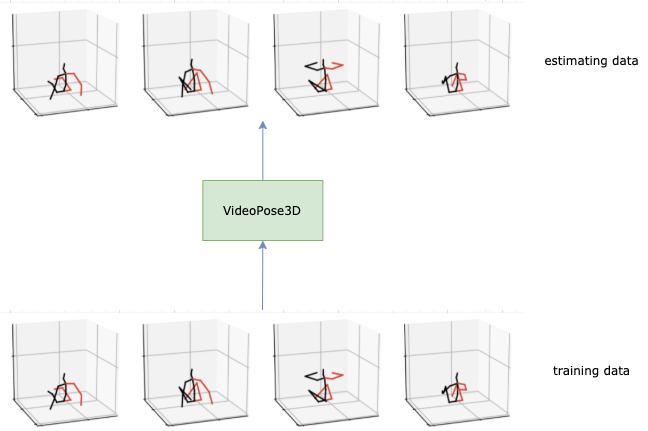
\includegraphics[scale=0.35]{model.png}}

%-------------------------------------------------------------------------
\subsection{Action-based Learning}

Compared to the original model we utilized a different data-processing approach. The original approach
mentioned in \textit{VideoPose3D} uses all actions in training data, and the estimating effect was good
overall. We utilize the method that we only take one type of action for training, and the total amount 
for training should be the same. Mathematically, take the action \textit{Sitting} for example, it can 
be expressed as

\begin{equation}
	\sum_{i\in actions}{f(i)} = f(Sitting)\cdot t
\end{equation}
where $f$ stands for the frames of subject, and $t$ means the number of epochs of our action-based 
training.

In this approach, we utilize only one time of action, which means we save more data; and we also produce
the results in the same time, the evidence can be illustrated by formula (1). After testing, we conclude 
that our work outperforms the original work by 11\%.

The principle of our work is shown below.

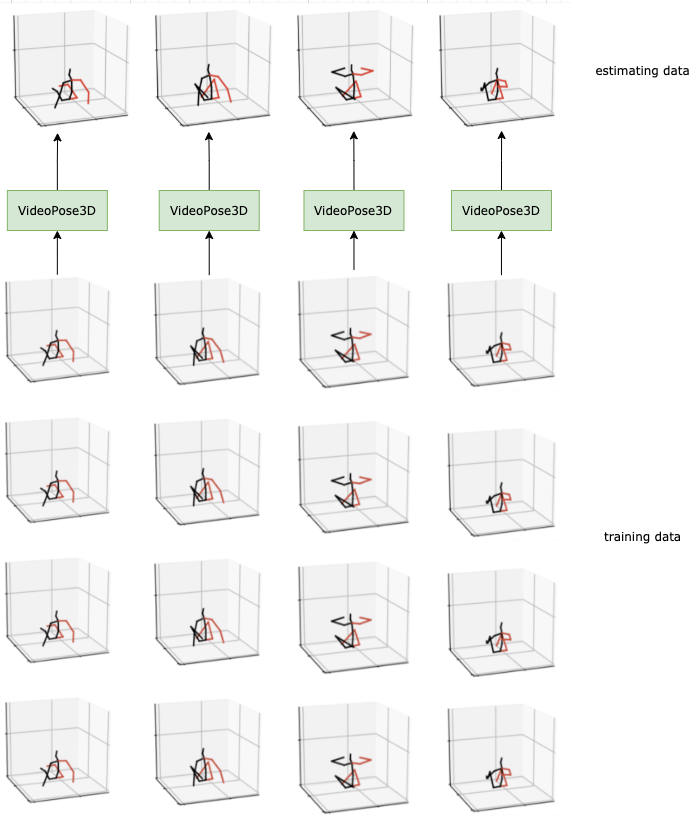
\includegraphics[scale=0.35]{model_new}

%------------------------------------------------------------------------
\section{Related Work}

Our work is based on the previous work \textit{VideoPose3D} with an inspiration for its
semi-supervised approach. Earlier work has shown the effect of semi-supervised learning
as a great way for improving training performance \cite{zhu2009introduction}. 

%-------------------------------------------------------------------------
\subsection{VideoPose3D}


\textit{VideoPose3D} is the current state-of-the-art approach which utilizes a fully 
convolutional model based on dilated temporal convolutions over 2D keypoints. 
\cite{pavlakos2017coarse,pavllo20193d}. In early researches the main solution
was to use recurrent neural networks (RNN) \cite{lee2018propagating}, but the research
group of \textit{VideoPose3D} utilized the convolutional neuron network (CNN) to gain
an efficient result on the dataset \textit{Human3.6M}, with the inspiration that
many authors had mentioned CNN in temporal models. Some researches has also shown the 
idea of using a spacial-temporal model being useful \cite{7298734}, but that's not utilized in our 
research.

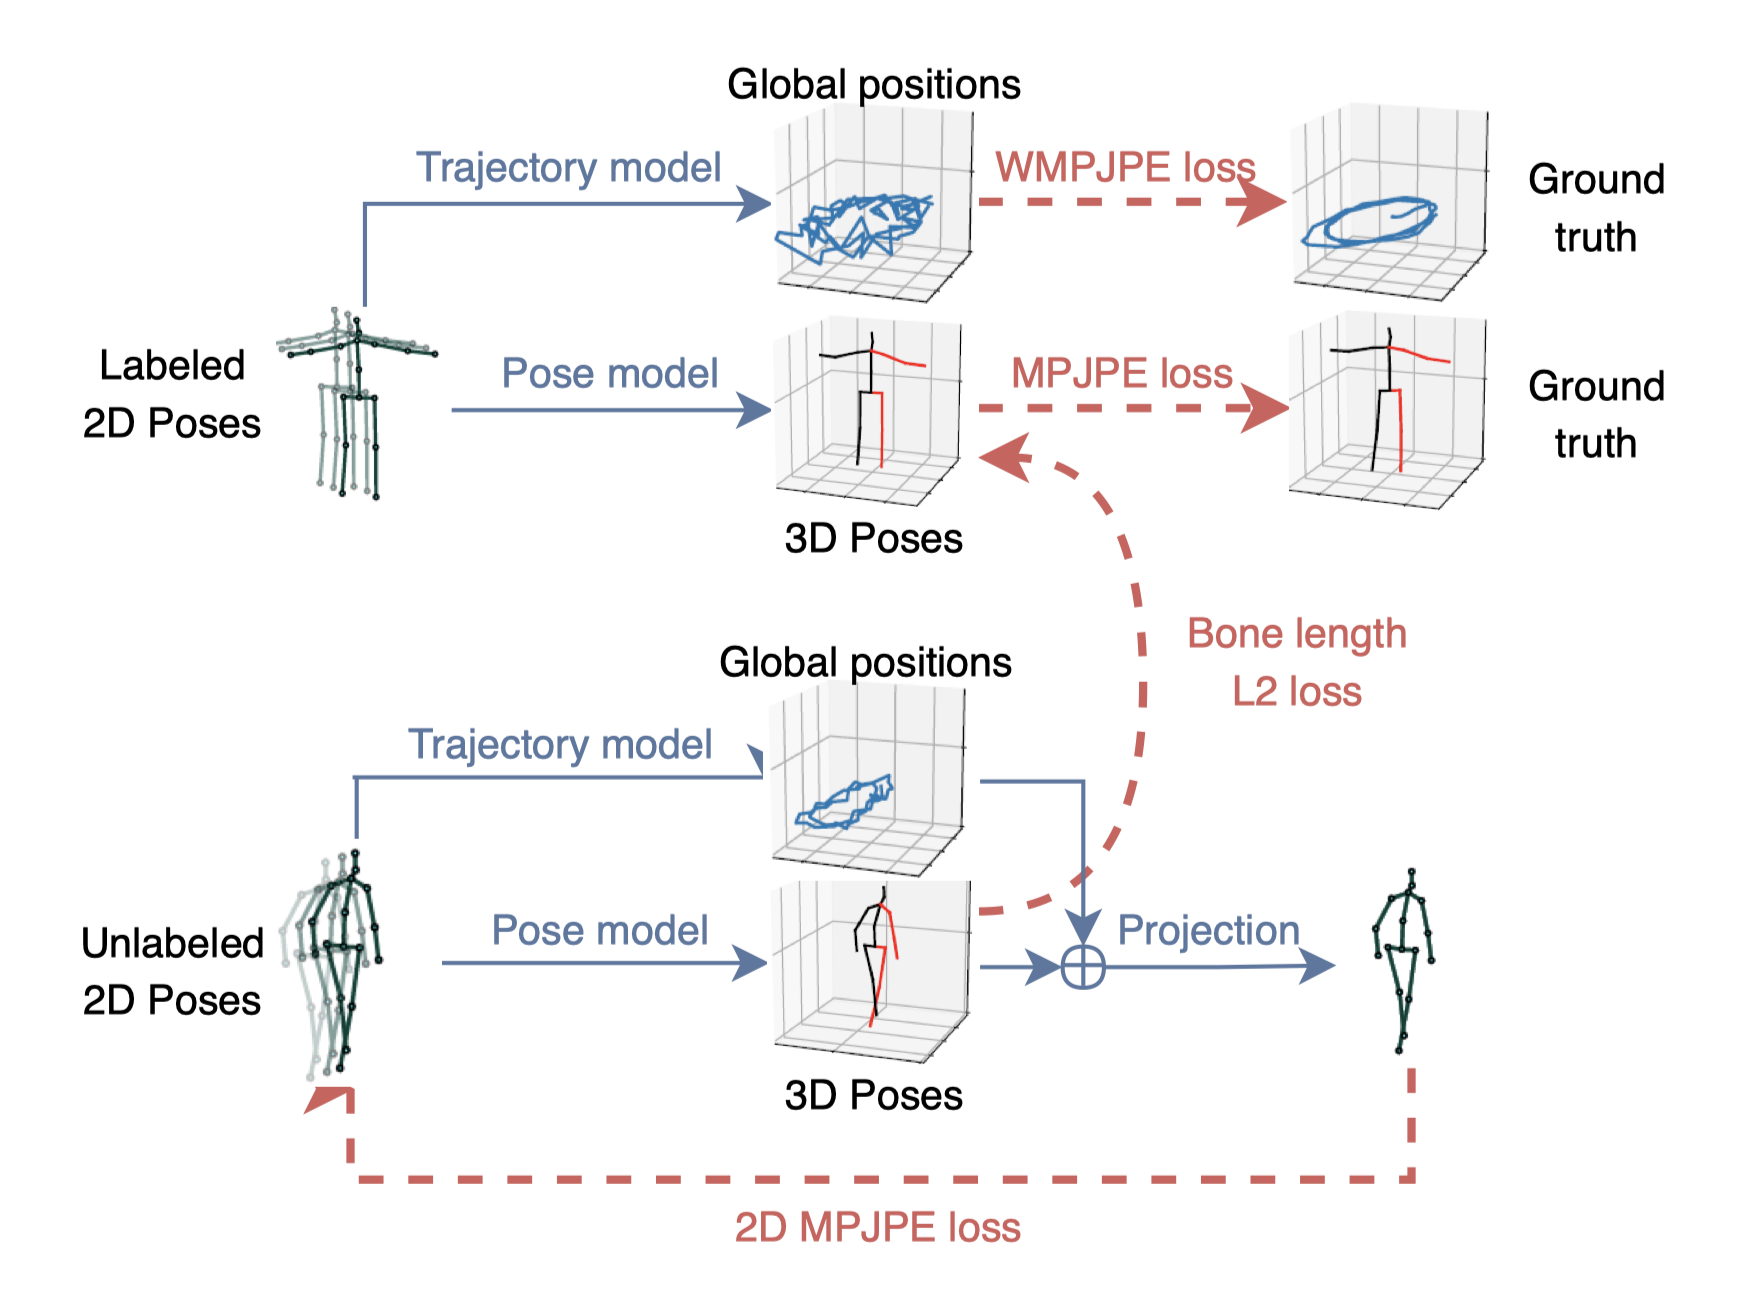
\includegraphics[scale=0.25]{original.png}



%-------------------------------------------------------------------------
\subsection{Action-based Learning}

The idea of homogenized learning was proposed firstly by Action Estimations \cite{yao2012coupled,wang2013action}.



%-------------------------------------------------------------------------
\subsection{Homography Estimation}

The idea of using homonegeious actions in a dataset was also inspired from Homography Estimation
in some deep images \cite{detone2016deep}. 



%------------------------------------------------------------------------
\section{Experimental Setup}

For the code of this project, please refer to the url below.

 \url{https://github.com/BiEchi/Pose3dDirectionalTraining}. 
 
The detailed experimental setup can also be explored in \textit{README.md} in the github repo. To reproduce
the results, you need to test for 15 times for each type of action, and it's preferable to test for multiple
times. It's more convenient to use \textit{bash} scripts to save time.

%------------------------------------------------------------------------

\section{Results}

Shown below are the results of the experiment. Expect a minor error when testing on your own. Note that all
unit are millimeter.

\subsection{Small Number of Epochs}

\begin{table}[H]
\caption{MPJPE, 3*3, unit-epoch}

\begin{tabular}{ccc}

\hline
Action & Original, MPJPE & Action-based, MPJPE\\
\hline

Eating&  56.34 & \textbf{52.07}\\
Sitting& 70.49 & 70.86\\

\hline
\end{tabular}
\end{table}


\begin{table}[H]
\caption{Velocity Error, 3*3, unit-epoch}


\begin{tabular}{ccc}
\hline
Action & Original, Velo-M  & Action-based, Velo-M\\
\hline

Eating&  3.14 & \textbf{3.01}\\
Sitting& 3.14 & \textbf{2.86}\\

\hline
\end{tabular}
\end{table}


\subsection{Large Number of Epochs}

For a large number of data, we observe that because of the characteristics of the model that \textit{VideoPose3D}
utilizes, the epoch refuses to increase after epoch 60 (i.e. epoch 4 of the original training method). 


\begin{table}[H]
\caption{Property Cluster, 3*3, 80-epoch}
\centering
\begin{tabular}{ccc}
\hline
Type & Original  & Eating-based\\
\hline

Time Consumed&  81173 sec & 56921 sec\\
MPJPE-Eating&  43.30 mm & 49.27 mm\\
Velo-M-Eating&  2.24 mm & 2.56 mm  \\

\hline
\end{tabular}
\end{table}

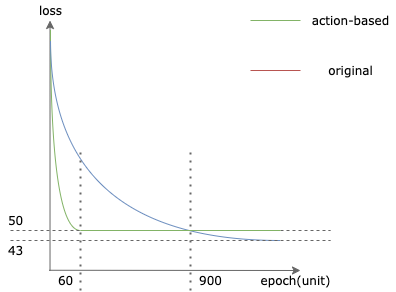
\includegraphics[scale=0.55]{training_epochs.png}



\section{Conclusion}
According to the results shown above, we conclude that the action-based model has a better performance on small epochs because 
they learn faster than the original one, though it has a worse performance on the top performance.


\newpage

{\small
\bibliographystyle{ieee_fullname}
\bibliography{egbib}
}

\end{document}

